% 
% Chickens, Anyone?  (BOOK version)
% (c) 2009 Eric R. Jeschke (eric@redskieatnight.com).
% This work is licensed under a Creative Commons Attribution-Share Alike
% 3.0 United States License
% See http://creativecommons.org/licenses/by-sa/3.0/us/
%
% Eric Jeschke makes no representation about the suitability or accuracy
% of this software or data for any purpose, and makes no warranties,
% either express or implied, including merchantability and fitness for a
% particular purpose or that the use of this software or data will not
% infringe any third party patents, copyrights, trademarks, or other
% rights.  The software and data are provided "as is". 
%
% 
% If you make a .sty file, please let me know!
%
% [top-level file]
\nonstopmode

\documentclass[10pt,final,openany]{book}
\usepackage{graphicx}
% where can I find the photos that will be imported for this version
\graphicspath{{./photos.book/}}

% font configuration is factored out
% Only uncomment if you have the fontspec package installed
% You will have to set the appropriate font names for what you have
% installed.
%
% You might be able to use opentype tools to find out the names of
% the fonts you can use here, or you can just experiment
%  $ otfinfo -a .../*.ttf
%
\usepackage{fontspec}
\setmainfont[Mapping=tex-text]{Garamond}
\setsansfont[Mapping=tex-text]{Arial}
\setmonofont[Mapping=tex-text]{Courier New}


% in case you want to embed any hyperlinks
% turn on colorlinks to avoid the nasty box around the link
\usepackage[colorlinks=true,urlcolor=black]{hyperref}

% geometry package is a much more reasonable way to set margins in LaTeX
% for Blurb, set this to the actual desired size as indicated by the
% size calculator on their web site
\usepackage[paperwidth=9.625in, paperheight=8.25in, 
            % amount we 'lose' (visually) due to the binding
            % left and right pages are offset a bit to the sides
            % (typically looks better for most kinds of bindings)
            bindingoffset=0.25in,
            % set total to the dimensions of the printed part
            total={8in,7.75in},
            % include header/footer/margin notes in printed area
            twoside, includeall, nomarginpar,
            ignorehead=false, ignorefoot=false, ignoremp=false,
            % center printed area on page
            vcentering, hcentering]{geometry}

% only play with these if you are going to do margin notes
% width of margin notes area
%\setlength{\marginparwidth}{0in}
% distance between margin and paragraph
%\setlength{\marginparsep}{0in}

% footer configuration 
\setlength{\footnotesep}{10pt}

% header configuration
\setlength{\headheight}{10pt}
\setlength{\headsep}{0.1in}

\title{Chickens, Anyone?}
\author{Eric Jeschke}

%%%%%%%%% PDF/X-3 stuff, necessary for Blurb IF USING pdflatex %%%%%%%%%
% ICC color profiles are embedded in the images
%% \pdfinfo{
%% /Title (Chickens, Anyone?)   % set your title here
%% /Author (Eric Jeschke)       % set author name
%% /Subject (Chickens)          % set subject
%% /Keywords (Chickens, Hawaii) % set keywords
%% /Trapped (False)
%% /GTS_PDFXVersion (PDF/X-3:2002)
%% }
%% % must have a trim box, but I think Blurb ignores the values
%% \pdfpageattr{%/MediaBox [0 0 693.36000 594.00000]
%% /TrimBox [0.00000 9.00000 684.36000 585.00000]}
%% \pdfminorversion=3
%% \pdfcatalog{
%% /OutputIntents [ <<
%% /Info (none)
%% /Type /OutputIntent
%% /S /GTS_PDFX
%% /OutputConditionIdentifier (Blurb.com)
%% /RegistryName (http://www.color.org/)
%% >> ]
%% }

%%%%%%%%% PDF/X-3 stuff, necessary for Blurb IF USING xelatex %%%%%%%%%
\special{pdf:docinfo <<
/Title (Chickens, Anyone?)   % set your title here
/Author (Eric Jeschke)       % set author name
/Subject (Chickens)          % set subject
/Keywords (Chickens, Hawaii) % set keywords
/Trapped (False)
/GTS_PDFXVersion (PDF/X-3:2002)
% must have a trim box, but I think Blurb ignores the values
/TrimBox [0.00000 9.00000 684.36000 585.00000] >>
}
\special{pdf:put @catalog <<
/OutputIntents [ <<
/Info (none)
/Type /OutputIntent
/S /GTS_PDFX
/OutputConditionIdentifier (Blurb.com)
/RegistryName (http://www.color.org/)
>> ] >>
}

% paragraph indentations
\setlength{\parindent}{0in}
% amount of space before each new paragraph begins
\setlength{\parskip}{1em}

% comment to force even justification
\raggedright

\begin{document}

\pagestyle{empty}

% interior facing page for book version
\vspace*{3in}
\begin{center}
{\Huge Chickens, Anyone?}

{\Large by Eric Jeschke}
\end{center}

\newpage

% bring in the rest of the content which is in common with the book
% version
%
% common information to the web version and book version
%
% images will be imported by searching the paths set with \graphicspath
% the book.tex or web.tex sets this so the correct resolution images end
% up in the correct document.
% 
% cover is done elsewhere, as this is usually broken out from the 
% ``text block'' for POD publishing--see book.tex
%

\vspace*{5in}
{\large Copyright (C) 2009 Lu Tao  All Rights Reserved.}

This book may not be reproduced in any form without written permission
of the author. 

{\tt 1417274896@qq.com}
\newpage

\vspace*{2in}
\begin{center}
{\LARGE For You}

{\large For auld lang syne}

\vspace*{0.5in}


\includegraphics[width=3in]{me_night.jpg}
\end{center}
\newpage

\vspace*{1in}
{\LARGE About this book}

I'm writing this book to practise {LaTeX} skills.


\vspace*{0.25in}

{\LARGE This boy is from the steppe.}

This boy is from the steppe.
I've speed most of my childhood in Hohhot, Inner Mongolia. 
The scene of the steppe in my hometown keeps flashing back in my mind these days.  
And it inspires me to make this album in memory of my past days.
These photographs represent some part of me. 
To some extent, to read this book is to read about this boy.

Although we have owned other kinds of critters through the years we had
never had chickens before, so this project was definitely one of
discovery. 
Thankfully, with sites like {\tt mypetchicken.com} and 
{\tt backyardchickens.com} to
guide us, as well as plenty of advice from friends and co-workers with
chickens, we're well on our way. This then, is the practical story of
how we went about it for the first month. Because you see, Solo Photo
Book Month doesn't wait for the full story of the chickens; there is
only time for the beginning of the story--all the photos have to be taken
in a 30 day period of time, and a book must be produced at the end.

And so, without further ado, 

{\Large {\em BacGawwwwk!!}}
\newpage

\vspace*{3in}
\begin{center}
\Huge{There's a hint of summer in the air.}
\end{center}
\newpage

\pagestyle{plain}

\vspace*{\fill}
\includegraphics[width=8in]{the70ceremany}

Next up, the chicks.  They had plenty of Rhode Island Reds on hand, but
\vspace*{\fill}
\newpage

\vspace*{\fill}
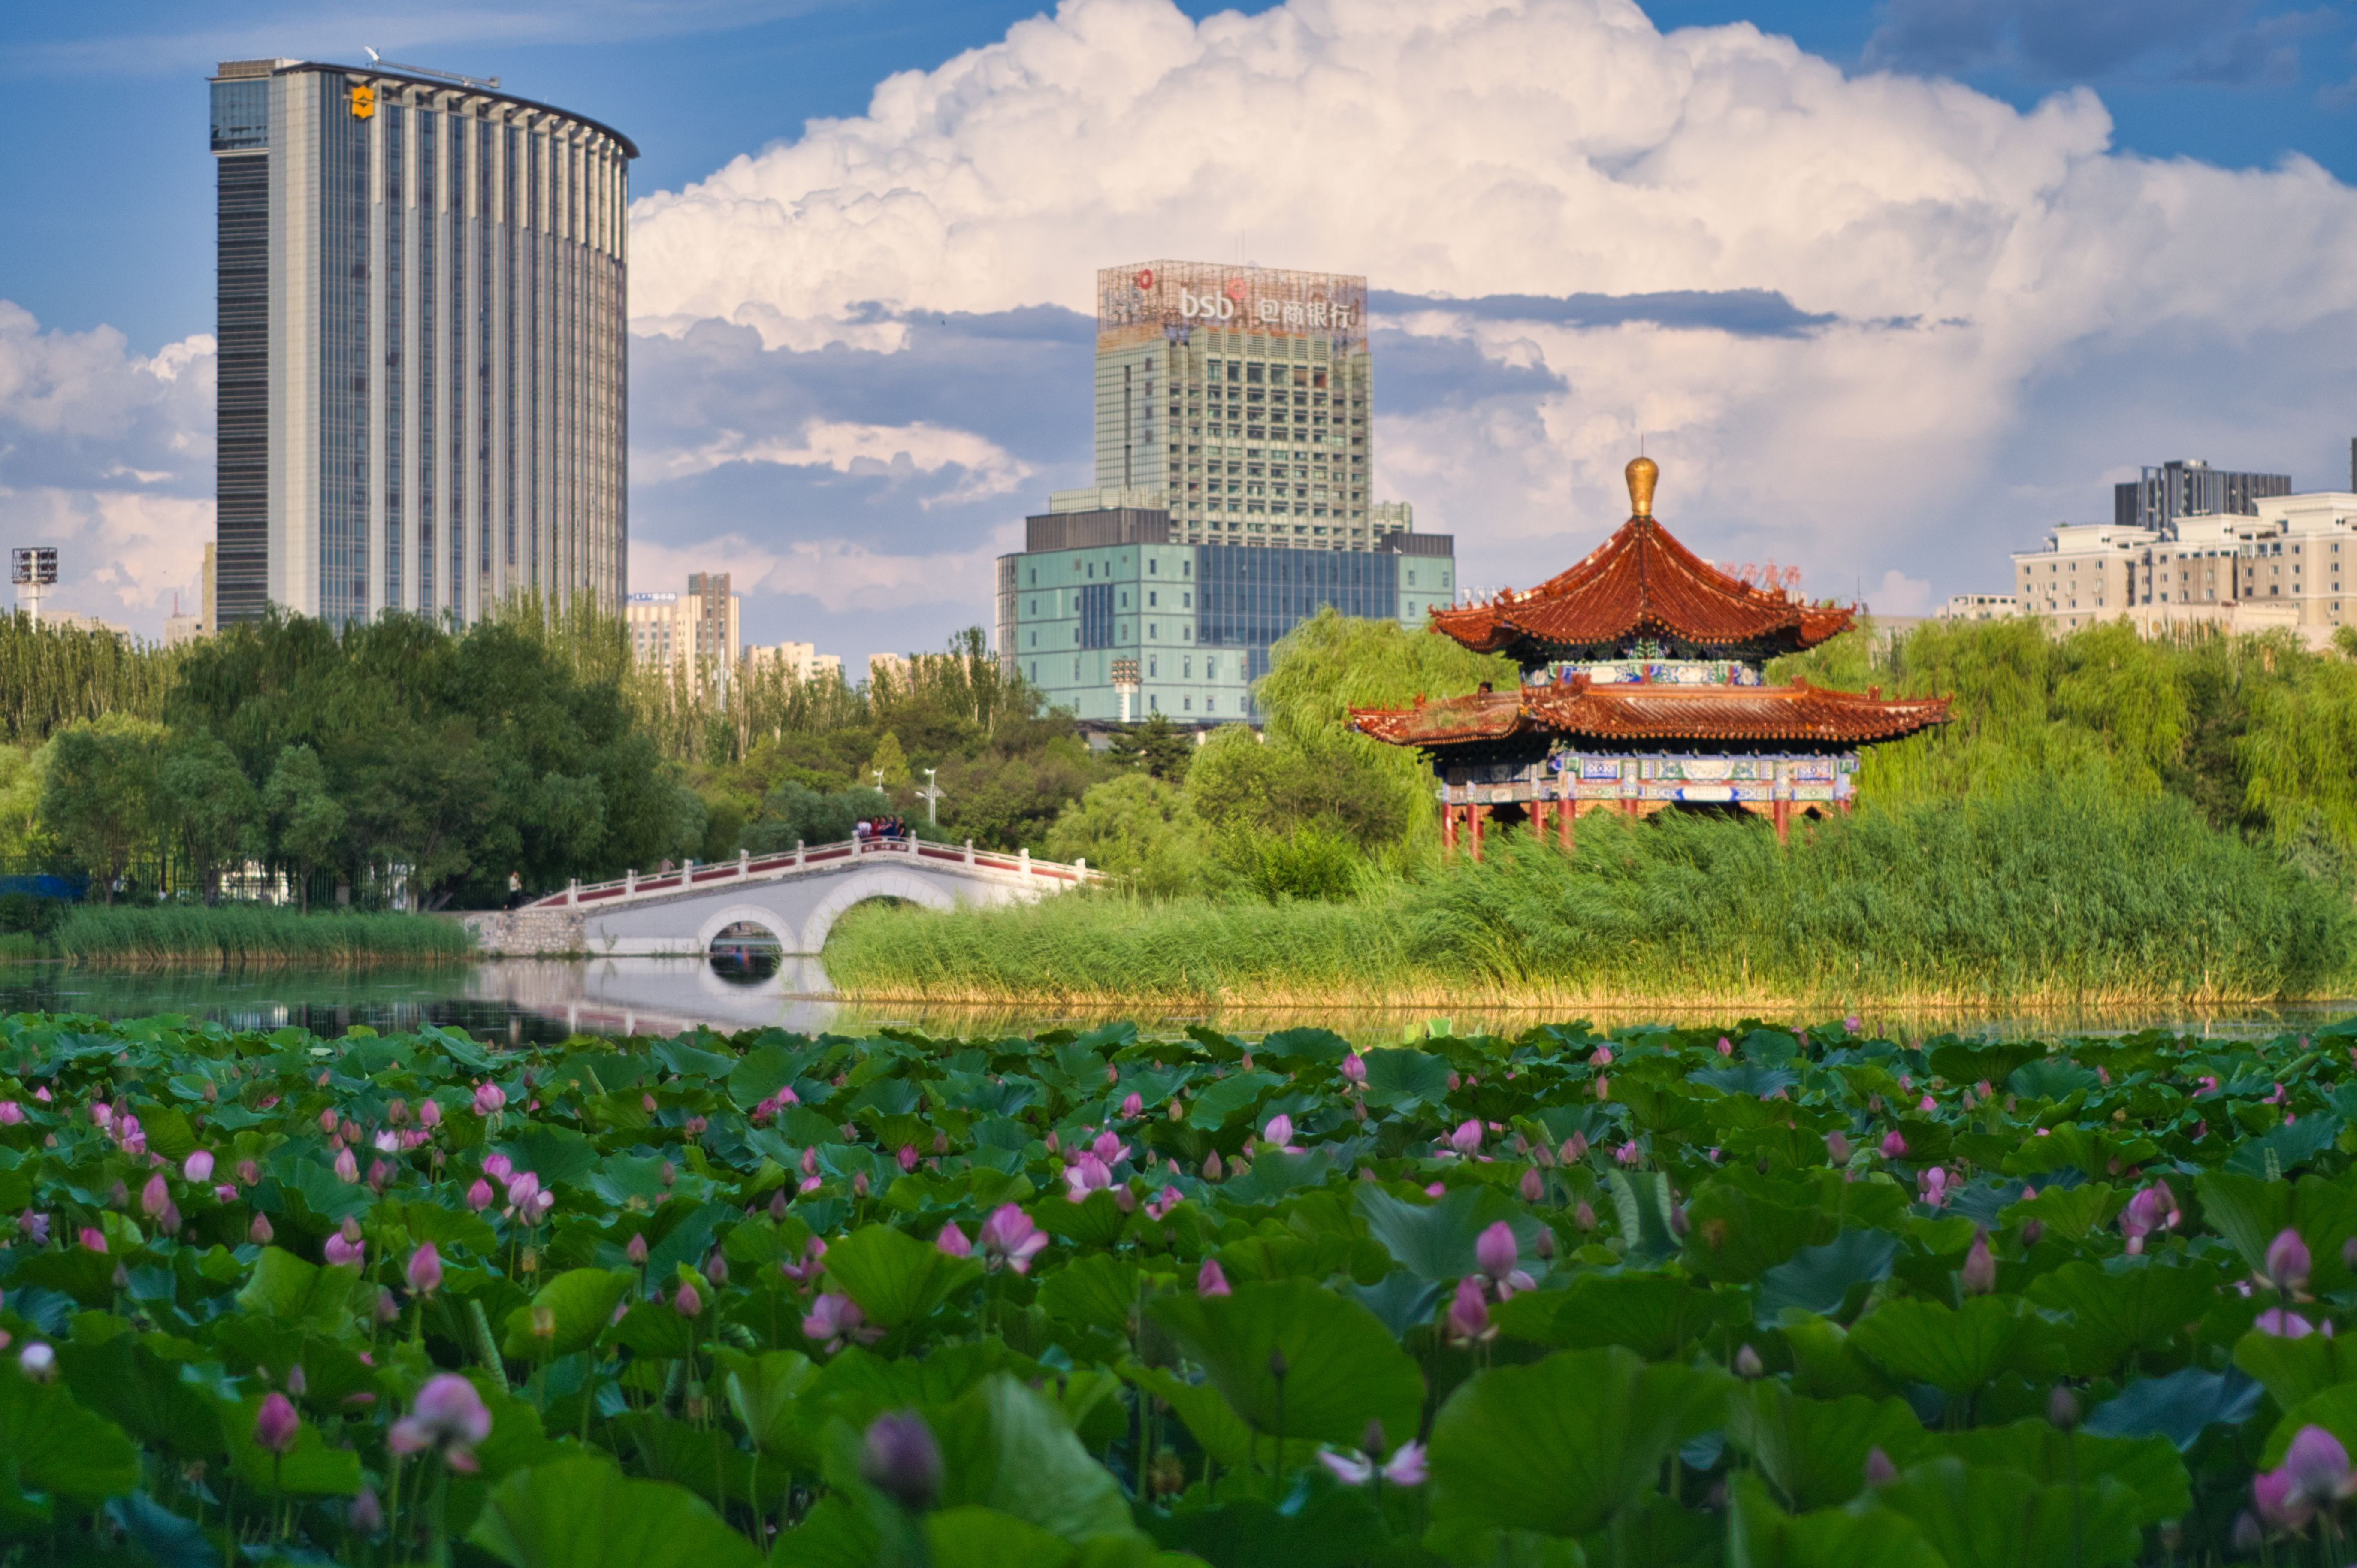
\includegraphics[width=8in]{theQingChengPart.jpg}

Before we brought anything home, I thought it might be a good idea to
figure out the where and how of a coop. It rains a fair bit here so I
\vspace*{\fill}
\newpage

\vspace*{\fill}
\includegraphics[width=8in]{the_Qingcheng_park_lake_in_spring}

First stop, supplies.  There was a large selection to choose from.  I
\vspace*{\fill}
\newpage

\vspace*{\fill}
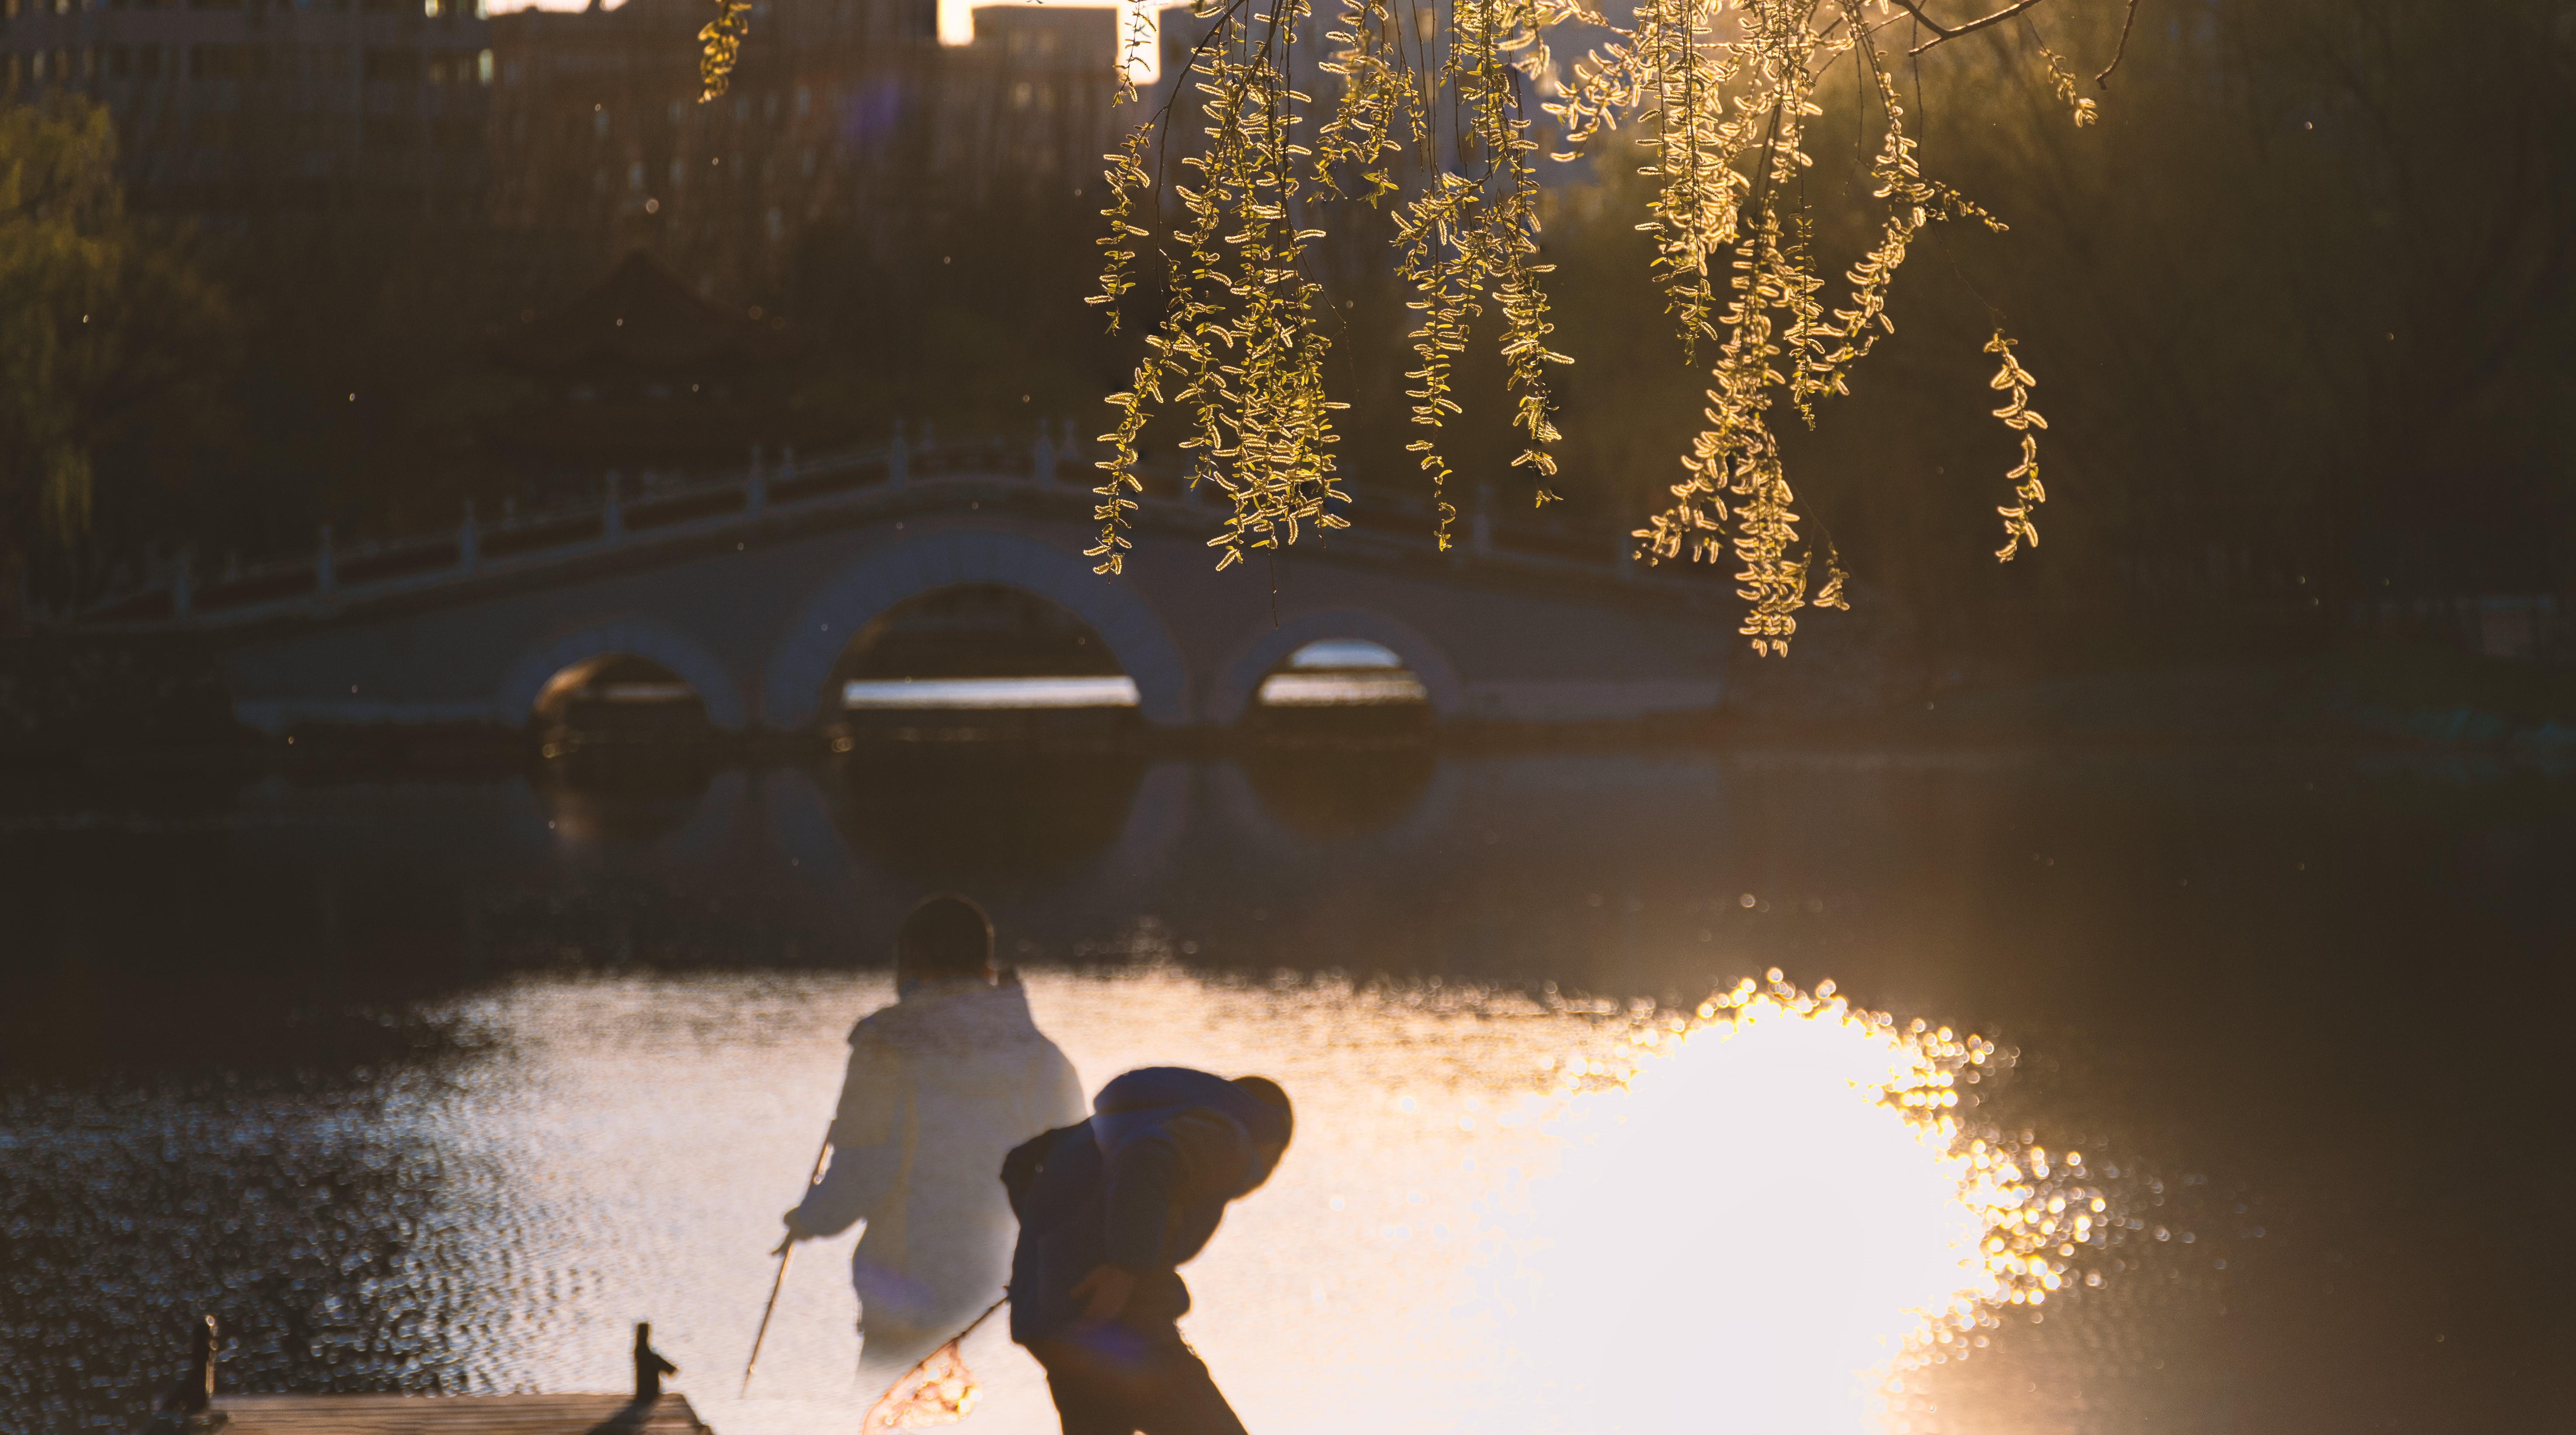
\includegraphics[width=8in]{thhfhjggjkh}

We went back to Del's a few days later, but the clerk informed me that
she'd sold the remainder of the chicks that morning to a single buyer,
and that they wouldn't be getting any more until next spring! Yikes! How
\vspace*{\fill}
\newpage

\vspace*{\fill}
\includegraphics[width=8in]{sounder_in_city.jpg}

On a late day in May we headed into town to Del's to pick up the chicks,
\vspace*{\fill}
\newpage

    \vspace*{\fill}
        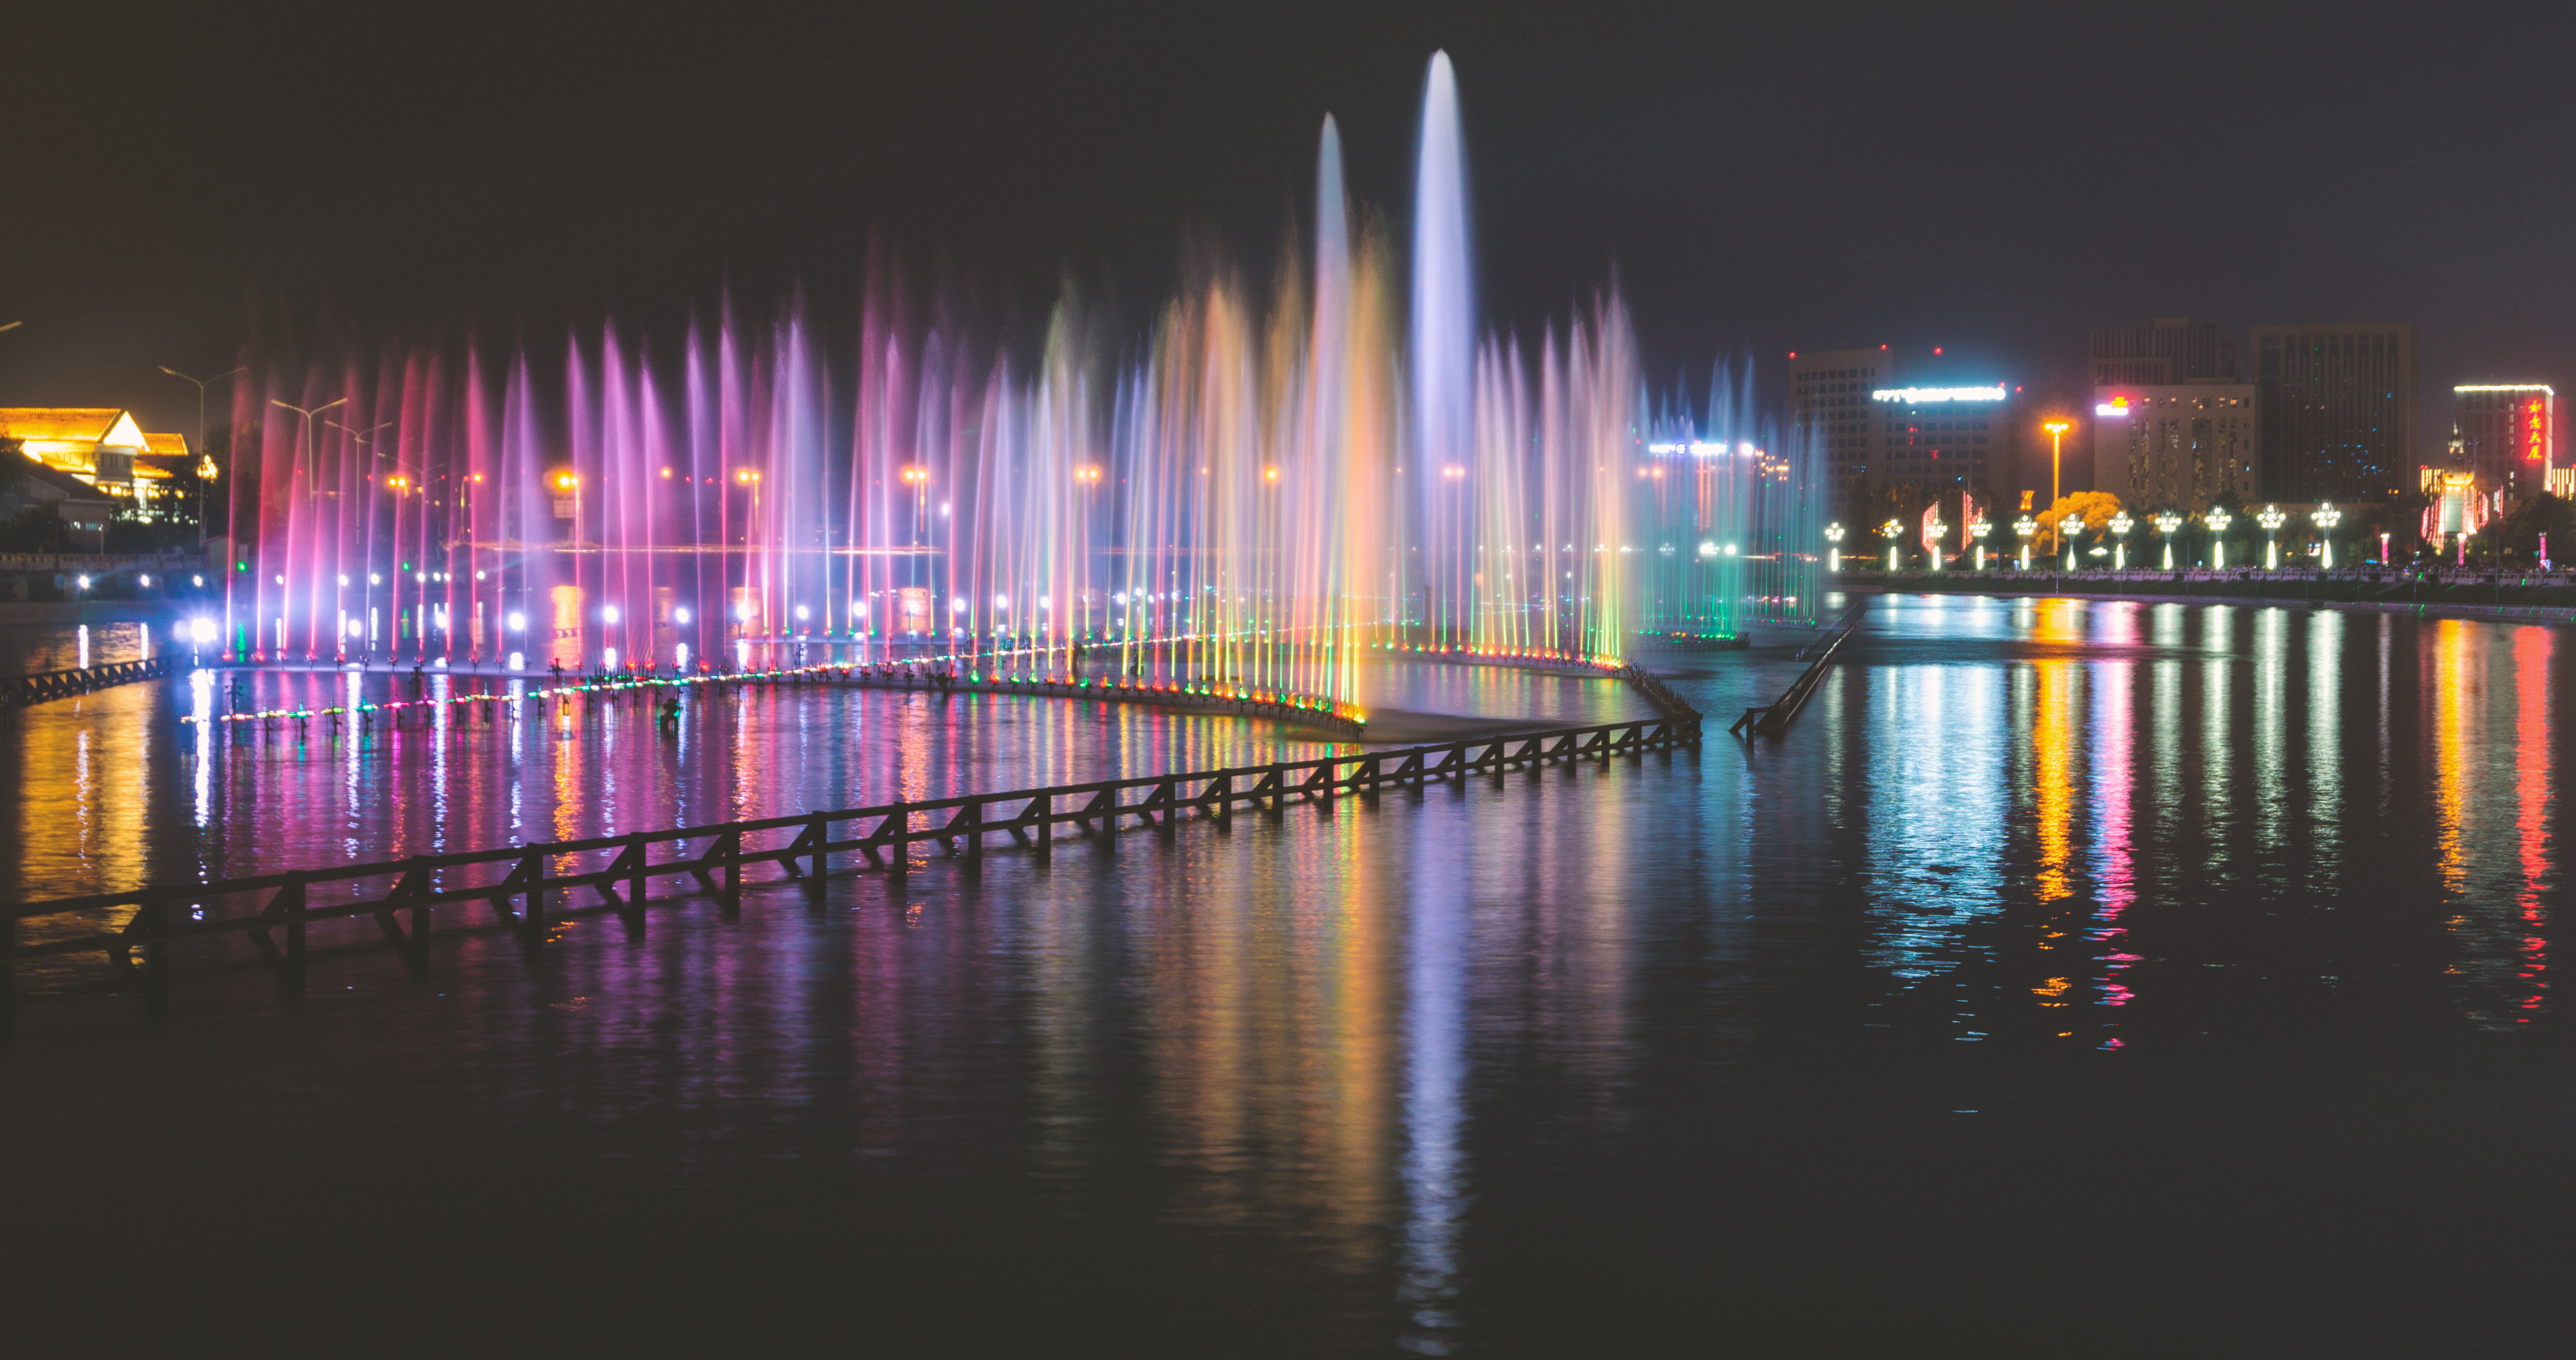
\includegraphics[width=8in]{ruyi_river_fangting}

        Next stop was Home Despot, er, Depot.  I had the beginnings of a plan in
        mind for a chicken coop.  My idea was to use a dog kennel as a starter
        coop.  HD had some inexpensive dog kennel kits, and I knew that with the
        galvanized steel I'd have something that could stand up to the rain, sun
        and termites.  I needed something to keep the chickens in, and predators
        out. 
    \vspace*{\fill}
\newpage

\vspace*{\fill}
\includegraphics[width=8in]{the_grocery}

The 6x6x4 kennel seemed about the right size for 6 chickens, which is
what I was targeting.  My calculations were that six would yield us a
decent number of eggs per week.  After some reconsideration, we put the
\vspace*{\fill}
\newpage

% \begin{center}{\Large ``Furrow'' }\end{center}

\vspace*{1in}

{\LARGE Book Considerations}

Solo Photo Book Month (sofobomo.org) is a DIY project to make a photo
book in one month. All of the photos must be taken and the book laid 
out and processed into a PDF in 31 days. This is my second year
participating in the event, along with many other photographers all over
the world. 
Last year I did square format B\&W, so I was determined to do color and
some sort of rectangular format this year. I chose to go all landscape, 
even though it meant passing on some good verticals I had taken. Also,
last year was more of a series of portraits, and this year I was
determined to have the book tell more of a story. I struggled to find
something that would fit my tight schedule this year when the ``chicken
project'', which I'd had on the back burner, hit me as a good fit to
dovetail with SoFoBoMo. 

If you have a comment to share, thoughts on the book, life with
chickens, technical info, questions, whatever...drop by 

\url{http://redskiesatnight.com/books/chickens-anyone}

and leave a comment. We'd love to hear from you! There you can also
download a PDF version. 

For more information about Solo Photo Book Month, visit

\url{http://sofobomo.org/}

\vspace*{0.25in}

{\LARGE Technical Details}

I was really pressed for time to get the book done in the requisite 30
days this year. I threw it together with snapshots taken with a Ricoh
GX100 camera. No post processing was done except for some quick levels
adjustments in the image editor GIMP.
{\em ImageMagick} was used to batch downsample the images for the web version
(144 dpi) or the book version (300 dpi). 
I designed the book using \LaTeX (with the wonderful {\em xetex} and
{\em xdvipdfmx}) for easier adjustments for dead tree publishing. 
The font used is Garamond. This book was made on Linux.

%END


\end{document}
